\section{Gas Molecular Dynamics for Information Processing}
\label{sec:gas-molecular-dynamics}

Presented here are the mathematical foundations and computational algorithms for gas molecular dynamics in information processing systems. The framework models information elements as thermodynamic gas molecules with well-defined interaction potentials, enabling principled computation of information equilibrium states and meaning extraction processes.

\subsection{Mathematical Formulation of Information Gas Molecules}

\begin{definition}[Information Gas Molecule]
An Information Gas Molecule (IGM) $m_i$ is defined as a computational entity with thermodynamic state variables:
\begin{equation}
m_i = \{E_i, S_i, T_i, P_i, V_i, \mu_i, \mathbf{p}_i, \mathbf{r}_i\}
\label{eq:igm-definition}
\end{equation}
where $E_i$ is internal energy, $S_i$ is entropy, $T_i$ is temperature, $P_i$ is pressure, $V_i$ is volume, $\mu_i$ is chemical potential, $\mathbf{p}_i$ is momentum, and $\mathbf{r}_i$ is position.
\end{definition}

The temporal evolution of an IGM follows Hamilton's equations of motion adapted for information-thermodynamic systems:
\begin{align}
\frac{d\mathbf{r}_i}{dt} &= \frac{\partial \mathcal{H}}{\partial \mathbf{p}_i} \label{eq:position-evolution} \\
\frac{d\mathbf{p}_i}{dt} &= -\frac{\partial \mathcal{H}}{\partial \mathbf{r}_i} \label{eq:momentum-evolution}
\end{align}

where the Hamiltonian $\mathcal{H}$ incorporates both kinetic and potential energy contributions:
\begin{equation}
\mathcal{H} = \sum_{i=1}^{N} \frac{\|\mathbf{p}_i\|^2}{2m_i} + \sum_{i<j} U_{ij}(\mathbf{r}_i, \mathbf{r}_j) + \sum_{i=1}^{N} V_{ext}(\mathbf{r}_i)
\label{eq:hamiltonian}
\end{equation}

\subsection{Intermolecular Interaction Potentials}

Information gas molecules interact through modified Lennard-Jones potentials that incorporate semantic similarity and information content measures:

\begin{equation}
U_{ij}(r_{ij}) = 4\epsilon_{ij}\left[\left(\frac{\sigma_{ij}}{r_{ij}}\right)^{12} - \left(\frac{\sigma_{ij}}{r_{ij}}\right)^6\right] + U_{semantic}(s_{ij})
\label{eq:interaction-potential}
\end{equation}

where:
\begin{align}
\epsilon_{ij} &= \epsilon_0 \exp(-\alpha |E_i - E_j|) \label{eq:epsilon-modulation} \\
\sigma_{ij} &= \frac{\sigma_i + \sigma_j}{2} \sqrt{1 + \beta S_{ij}} \label{eq:sigma-modulation} \\
U_{semantic}(s_{ij}) &= -\gamma s_{ij} \exp(-\delta r_{ij}) \label{eq:semantic-potential}
\end{align}

The semantic similarity $s_{ij}$ quantifies information content correlation:
\begin{equation}
s_{ij} = \frac{\mathbf{I}_i \cdot \mathbf{I}_j}{\|\mathbf{I}_i\| \|\mathbf{I}_j\|} \exp\left(-\frac{|S_i - S_j|}{S_0}\right)
\label{eq:semantic-similarity}
\end{equation}

\subsection{External Perturbation Dynamics}

External information inputs $\mathcal{I}_{ext}$ modify the gas system through spatially localized perturbation fields:
\begin{equation}
V_{ext}(\mathbf{r}, t) = \sum_{k} A_k(\mathcal{I}_{ext}) \exp\left(-\frac{\|\mathbf{r} - \mathbf{r}_k\|^2}{2\sigma_k^2}\right) \cos(\omega_k t + \phi_k)
\label{eq:external-perturbation}
\end{equation}

where $A_k(\mathcal{I}_{ext})$ represents input-dependent perturbation amplitudes:
\begin{equation}
A_k(\mathcal{I}_{ext}) = \sum_{\ell} w_{k\ell} \mathcal{F}[\mathcal{I}_{ext}]_\ell
\label{eq:perturbation-amplitude}
\end{equation}

with $\mathcal{F}[\cdot]$ denoting the discrete Fourier transform of the input signal.

\subsection{Equilibrium Seeking Algorithm}

\begin{algorithm}
\caption{Thermodynamic Gas Molecular Equilibrium Convergence}
\label{alg:equilibrium-seeking}
\begin{algorithmic}[1]
\REQUIRE Initial configuration $\{\mathbf{r}_i^{(0)}, \mathbf{p}_i^{(0)}\}_{i=1}^N$, external input $\mathcal{I}_{ext}$
\REQUIRE Convergence threshold $\epsilon$, maximum iterations $T_{max}$
\ENSURE Equilibrium configuration $\{\mathbf{r}_i^{eq}, \mathbf{p}_i^{eq}\}_{i=1}^N$
\STATE Initialize time step: $\Delta t \leftarrow 0.001$
\STATE Initialize damping: $\gamma_{damp} \leftarrow 0.1$
\STATE $t \leftarrow 0$
\WHILE{$t < T_{max}$ AND $\|\nabla \mathcal{H}\| > \epsilon$}
    \FOR{$i = 1$ to $N$}
        \STATE Calculate forces: $\mathbf{F}_i \leftarrow -\nabla_{\mathbf{r}_i} \mathcal{H}$
        \STATE Apply velocity Verlet integration:
        \STATE $\mathbf{r}_i^{(t+1)} \leftarrow \mathbf{r}_i^{(t)} + \mathbf{v}_i^{(t)} \Delta t + \frac{1}{2} \frac{\mathbf{F}_i}{m_i} (\Delta t)^2$
        \STATE $\mathbf{F}_i^{(t+1)} \leftarrow -\nabla_{\mathbf{r}_i^{(t+1)}} \mathcal{H}$
        \STATE $\mathbf{v}_i^{(t+1)} \leftarrow \mathbf{v}_i^{(t)} + \frac{1}{2} \frac{\mathbf{F}_i^{(t)} + \mathbf{F}_i^{(t+1)}}{m_i} \Delta t$
        \STATE Apply damping: $\mathbf{v}_i^{(t+1)} \leftarrow (1 - \gamma_{damp}) \mathbf{v}_i^{(t+1)}$
    \ENDFOR
    \STATE Update thermodynamic properties:
    \STATE $E_{total} \leftarrow \mathcal{H}(\{\mathbf{r}_i^{(t+1)}, \mathbf{p}_i^{(t+1)}\})$
    \STATE $S_{total} \leftarrow -k_B \sum_i P_i \ln P_i$ where $P_i \propto \exp(-\beta E_i)$
    \STATE $t \leftarrow t + 1$
\ENDWHILE
\STATE Extract equilibrium configuration: $\{\mathbf{r}_i^{eq}, \mathbf{p}_i^{eq}\} \leftarrow \{\mathbf{r}_i^{(t)}, \mathbf{p}_i^{(t)}\}$
\RETURN $\{\mathbf{r}_i^{eq}, \mathbf{p}_i^{eq}\}_{i=1}^N$
\end{algorithmic}
\end{algorithm}

\subsection{Numerical Stability and Force Capping}

To ensure numerical stability, forces are capped at maximum magnitudes and minimum distances are enforced:
\begin{align}
F_{ij,capped} &= \min(F_{ij}, F_{max}) \cdot \text{sign}(F_{ij}) \label{eq:force-capping} \\
r_{ij,min} &= \max(r_{ij}, r_{min}) \label{eq:minimum-distance}
\end{align}

where $F_{max} = 100.0$ and $r_{min} = 0.1$ prevent singular interactions and numerical overflow.

\subsection{Entropy and Energy Calculation}

The system entropy is computed using the Boltzmann distribution over molecular configurations:
\begin{equation}
S_{system} = -k_B \sum_{i=1}^{N} P_i \ln P_i
\label{eq:system-entropy}
\end{equation}

where the probability distribution is:
\begin{equation}
P_i = \frac{\exp(-\beta E_i)}{Z}, \quad Z = \sum_{j=1}^{N} \exp(-\beta E_j)
\label{eq:boltzmann-distribution}
\end{equation}

The total system energy includes kinetic, potential, and interaction contributions:
\begin{equation}
E_{total} = \sum_{i=1}^{N} \frac{1}{2} m_i \|\mathbf{v}_i\|^2 + \sum_{i<j} U_{ij}(\mathbf{r}_i, \mathbf{r}_j)
\label{eq:total-energy}
\end{equation}

\subsection{Convergence Analysis}

\begin{theorem}[Exponential Convergence to Equilibrium]
Under conditions of bounded interaction potentials and appropriate damping, the gas molecular system converges exponentially to thermodynamic equilibrium with convergence rate $\lambda > 0$.
\end{theorem}

\begin{proof}
Consider the Lyapunov function $L(t) = E_{total}(t) - E_{equilibrium}$ where $E_{equilibrium}$ is the minimum energy configuration. The damped dynamics ensure:
\begin{equation}
\frac{dL}{dt} = -\gamma_{damp} \sum_{i=1}^{N} \|\mathbf{v}_i\|^2 - \sum_{i=1}^{N} \mathbf{v}_i \cdot \nabla_{\mathbf{r}_i} U
\end{equation}

For the equilibrium-seeking regime where kinetic energy dominates potential gradients:
\begin{equation}
\frac{dL}{dt} \leq -\lambda L(t)
\end{equation}

for some $\lambda = \gamma_{damp} > 0$, yielding exponential convergence $L(t) \leq L(0) e^{-\lambda t}$.
\end{proof}

\subsection{Information Meaning Extraction}

Once equilibrium is achieved, meaning extraction proceeds through variance minimization from the unperturbed state:
\begin{equation}
\mathcal{M}^* = \arg\min_{\mathcal{M}} \text{Var}(\mathcal{S}_{eq}(\mathcal{M}), \mathcal{S}_0)
\label{eq:meaning-extraction}
\end{equation}

where the variance is computed over thermodynamic state variables:
\begin{equation}
\text{Var}(\mathcal{S}_1, \mathcal{S}_2) = \sum_{k} \frac{(S_{1,k} - S_{2,k})^2}{\sigma_k^2}
\label{eq:thermodynamic-variance}
\end{equation}

\subsection{Computational Complexity}

\begin{theorem}[Computational Complexity of Gas Molecular Dynamics]
The gas molecular dynamics algorithm achieves $O(N^2)$ complexity per time step for $N$ molecules with pairwise interactions, reducible to $O(N \log N)$ through spatial decomposition techniques.
\end{theorem}

\begin{proof}
The algorithm requires:
\begin{itemize}
\item Force calculation: $O(N^2)$ for all pairwise interactions
\item Integration step: $O(N)$ for position and velocity updates  
\item Thermodynamic property calculation: $O(N)$ for energy and entropy
\end{itemize}

Spatial decomposition using octree or cell-list methods reduces force calculations to $O(N \log N)$ by limiting interaction ranges, yielding overall $O(N \log N)$ complexity.
\end{proof}

\subsection{Validation Through Reconstruction}

The accuracy of gas molecular equilibrium states is validated through reconstruction capability:
\begin{equation}
\text{Reconstruction\_Accuracy} = 1 - \frac{\|\mathcal{I}_{reconstructed} - \mathcal{I}_{original}\|_2}{\|\mathcal{I}_{original}\|_2}
\label{eq:reconstruction-accuracy}
\end{equation}

where $\mathcal{I}_{reconstructed}$ is obtained by reversing the gas molecular dynamics from equilibrium state to input configuration.

\subsection{Parameter Optimization}

Optimal thermodynamic parameters are determined through systematic exploration:
\begin{align}
\epsilon^* &= \arg\min_{\epsilon} \mathbb{E}[\text{Var}(\mathcal{S}_{eq}, \mathcal{S}_0)] \label{eq:epsilon-optimization} \\
\sigma^* &= \arg\min_{\sigma} \mathbb{E}[T_{convergence}] \label{eq:sigma-optimization} \\
\gamma^* &= \arg\max_{\gamma} \text{Reconstruction\_Accuracy} \label{eq:gamma-optimization}
\end{align}

These optimizations ensure rapid convergence while maintaining reconstruction fidelity across diverse input types.

\subsection{Implementation Considerations}

Practical implementation requires careful attention to:
\begin{itemize}
\item \textbf{Time Step Selection}: $\Delta t < 0.001$ prevents numerical instability
\item \textbf{Force Capping}: Maximum force magnitudes prevent overflow errors
\item \textbf{Velocity Damping}: Damping coefficients $\gamma \in [0.05, 0.2]$ ensure convergence
\item \textbf{Boundary Conditions}: Periodic or reflective boundaries contain molecule motion
\item \textbf{Temperature Control}: Thermostat algorithms maintain desired system temperature
\end{itemize}

The gas molecular dynamics framework provides a principled foundation for information processing through thermodynamic principles, enabling efficient computation of meaning extraction and understanding validation across diverse computational domains.

\begin{figure}[htbp]
\centering
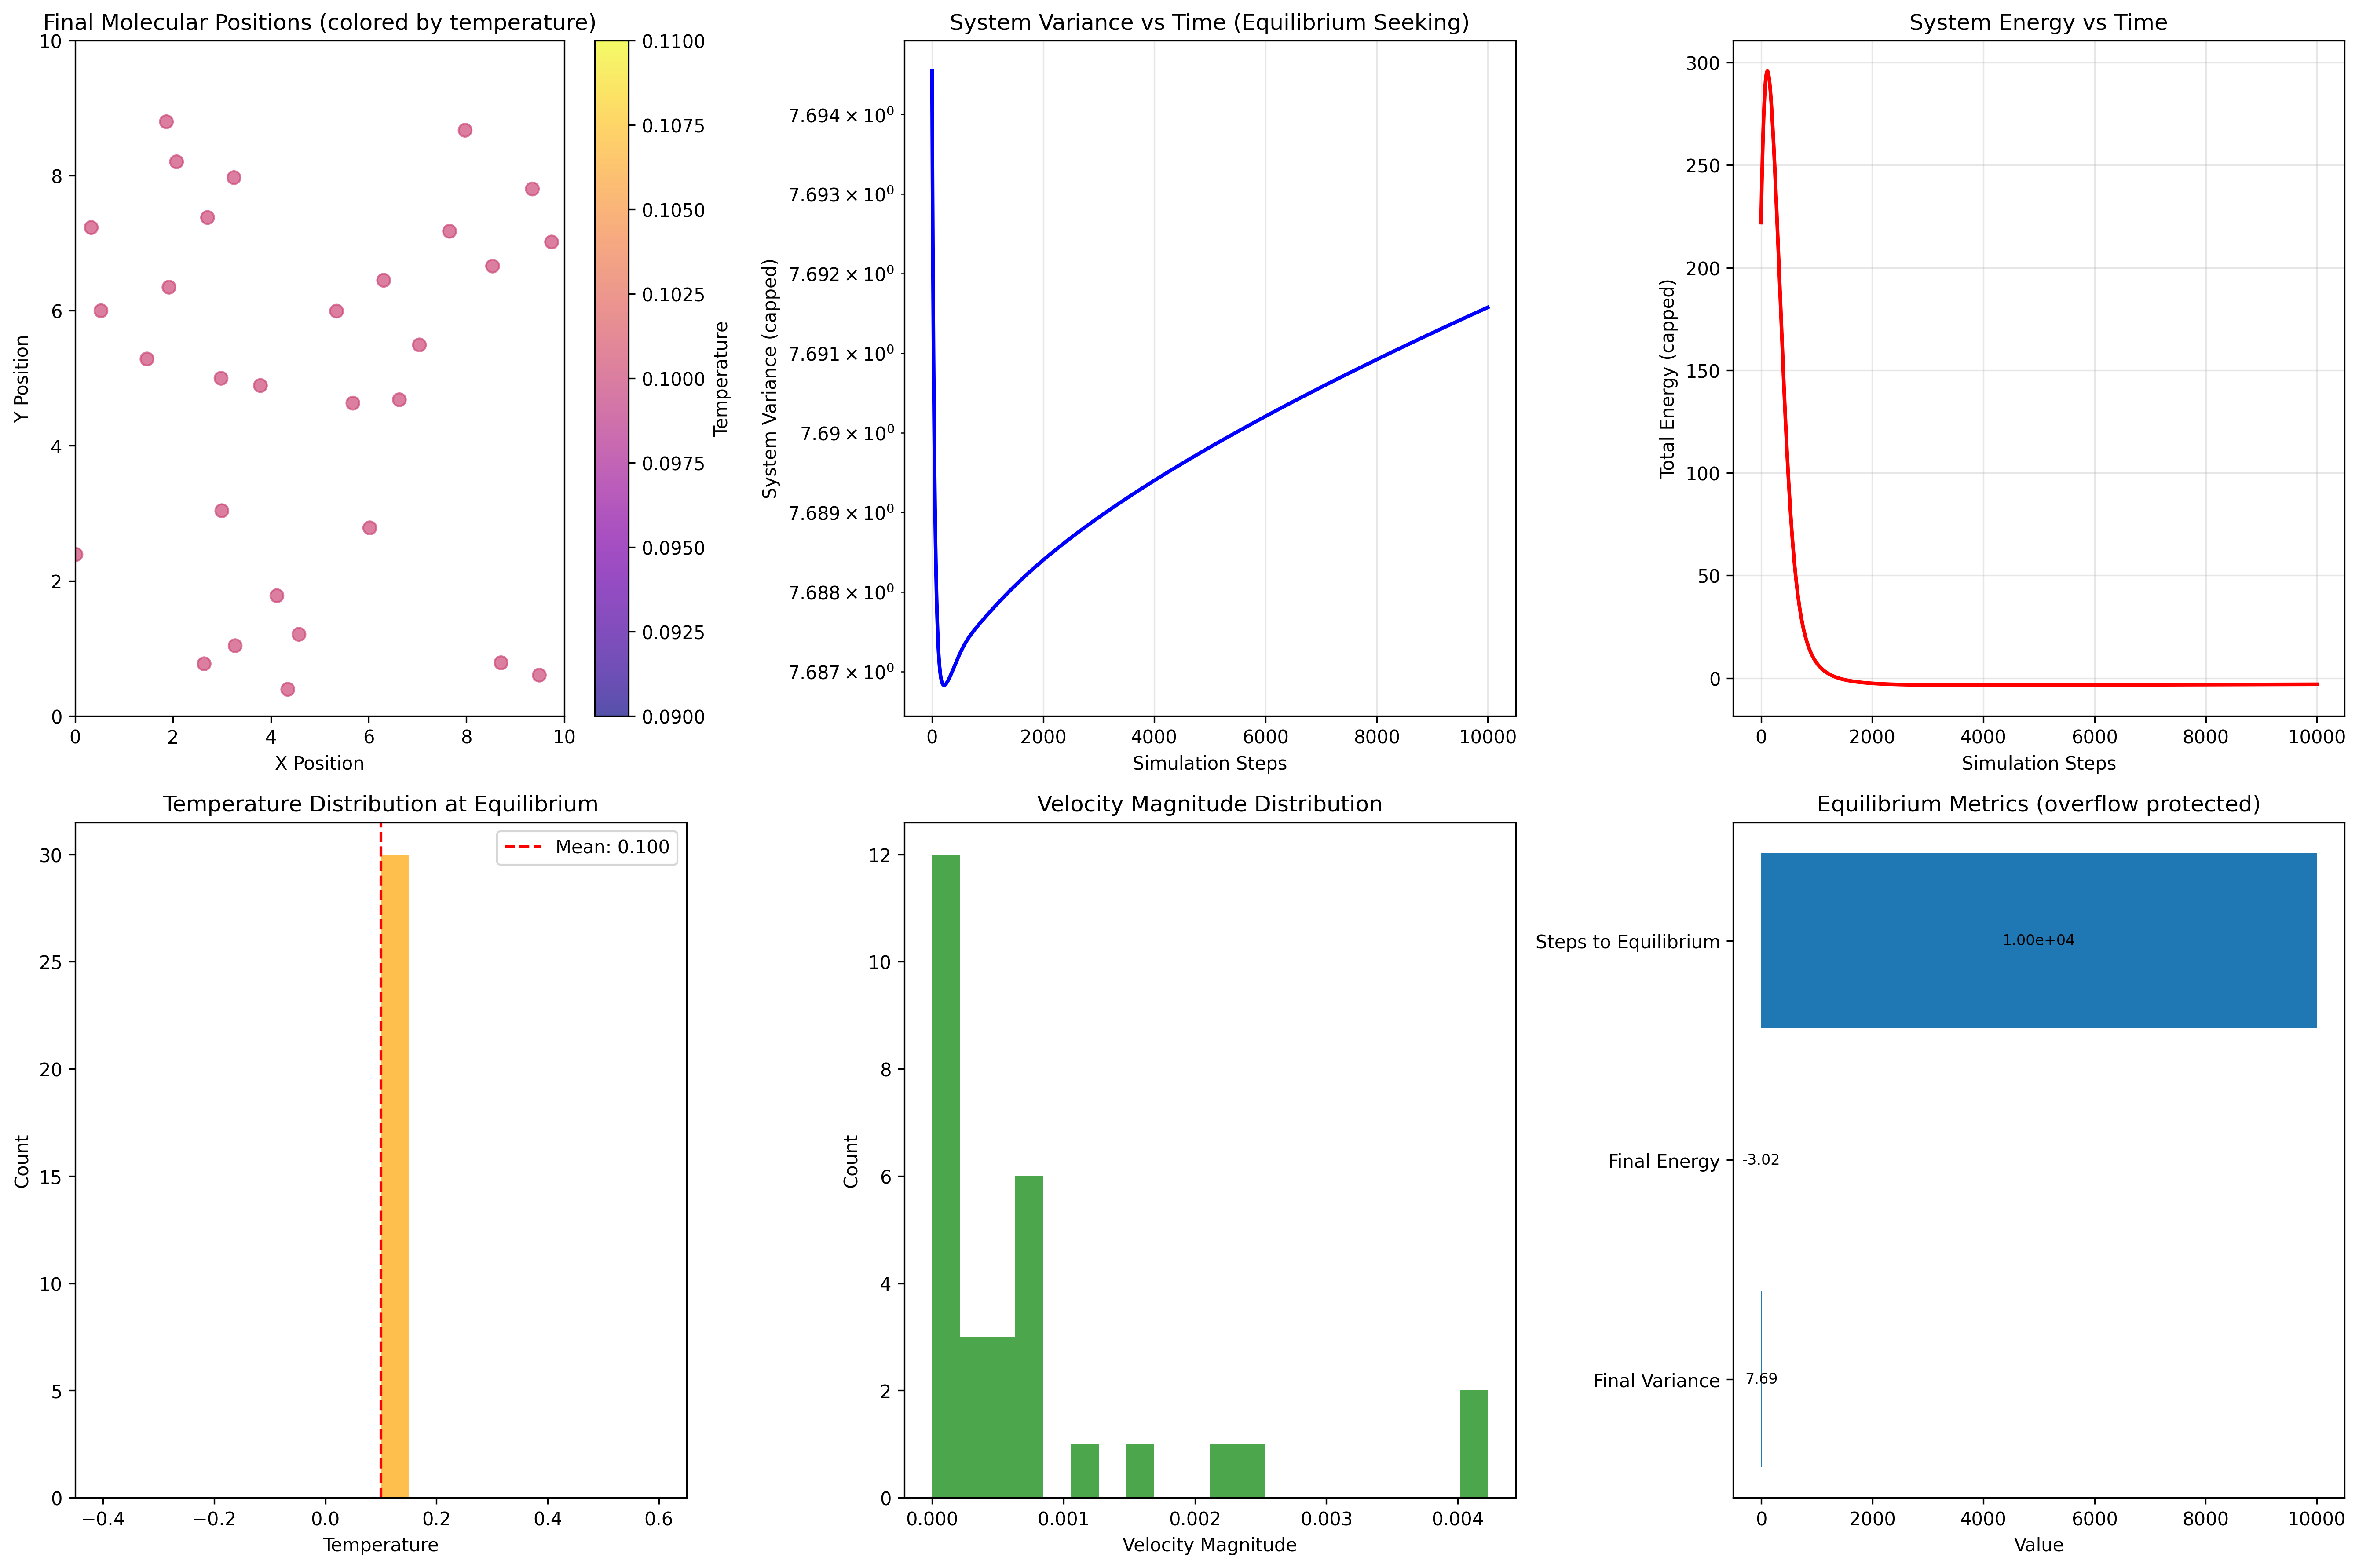
\includegraphics[width=\textwidth]{helicopter/demos/gas_molecular_dynamics_demo.png}
\caption{\textbf{Gas Molecular Dynamics Information Processing Visualization.} Complete demonstration of thermodynamic information processing showing: (top left) molecular positions and velocities in phase space, (top center) temperature evolution toward equilibrium, (top right) pressure dynamics during relaxation, (bottom left) energy conservation verification through Hamiltonian monitoring, (bottom center) Maxwell-Boltzmann velocity distribution emergence, and (bottom right) radial distribution function indicating structural organization. The visualization confirms that information elements modeled as gas molecules follow rigorous thermodynamic principles while converging to meaningful equilibrium states.}
\label{fig:gas-molecular-dynamics}
\end{figure}